\section{Results}

\begin{sansmath}
\sessionpy{pytex_subfigs(
        [
                {'script':'scripts/taskgroup.py', 'conf':'article/2x1.conf', 'options_pre':'{.48\\textwidth}',
                        'caption':'Task group comparison for animals targeted at all explored combinations of implant coordinates.',
                        'label':'mvt',
                        },
                {'script':'scripts/implant_coordinates_block.py', 'conf':'article/2x1_coordinates.conf', 'options_pre':'{.48\\textwidth}',
                        'caption':'Implant coordinate comparison for block stimulation trials (inner dots indicate best category group).',
                        'label':'mvib',
                        },
                ],
        caption='
                \\textbf{VTA activation is sensitive to the stimulation protocol category and the implant coordinates, with different trends in block and phasic stimulation trials.}
                Depicted are multifactorial (protocol and implant coordinates) comparisons of signal intensity in the VTA region of interest.
                Abbreviations:
                n (sample size),
                PA (posteroanterior),
                rel. (relative to).
                ',
        label='fig:mv',
        )}
\end{sansmath}

\begin{sansmath}
\sessionpy{pytex_subfigs(
        [
                {'script':'scripts/map_block_filtered_controlled.py', 'conf':'article/2asymetric_map.conf',
                        'options_pre':'{.39\\textwidth}',
                        'options_pre_caption':'\\vspace{-.5em}',
                        'caption':'Second-level t-statistic map for block-stimulus-evoked activity in best implant group animals (corrected for the wild type control response).\\vspace{.5em}',
                        'label':'mbfc',
                        },
                {'script':'scripts/distributions_block_filtered_controlled.py', 'conf':'article/2asymetric_distributions.conf',
                        'options_pre':'{.595\\textwidth}\\vspace{-.4em}',
                        'options_pre_caption':'\\vspace{-2em}',
                        'caption':'Distribution densities of statistic values from block-stimulus-evoked activity analysis in best implant group animals (corrected for the wildtype control response). Depicted are the 10 most strongly activated areas.',
                        'label':'dbfc',
                        },
                {'script':'scripts/map_block_other_controlled.py', 'conf':'article/2asymetric_map.conf',
                        'options_pre':'{.39\\textwidth}',
                        'options_pre_caption':'\\vspace{-.5em}',
                        'caption':'Second-level t-statistic map for block-stimulus-evoked activity in rejected implant group animals (corrected for the wild type control response).\\vspace{.5em}',
                        'label':'mboc',
                        },
                {'script':'scripts/distributions_block_other_controlled.py', 'conf':'article/2asymetric_distributions.conf',
                        'options_pre':'{.595\\textwidth}\\vspace{-.4em}',
                        'options_pre_caption':'\\vspace{-2em}',
                        'caption':'Distribution densities of statistic values from block-stimulus-evoked activity analysis in rejected implant group animals (corrected for the wild type control response). Depicted are the 10 most strongly activated areas.',
                        'label':'dboc',
                        },
                {'script':'scripts/map_block_filtered_seed.py', 'conf':'article/2asymetric_map.conf',
                        'options_pre':'{.39\\textwidth}',
                        'options_pre_caption':'\\vspace{-.5em}',
                        'caption':'Second-level t-statistic map for VTA seed-based functional connectivity during block stimulation in best implant group animals (VTA region in green).\\vspace{.5em}',
                        'label':'mbfs',
                        },
                {'script':'scripts/distributions_block_filtered_seed.py', 'conf':'article/2asymetric_distributions.conf',
                        'options_pre':'{.595\\textwidth}\\vspace{-.4em}',
                        'options_pre_caption':'\\vspace{-2em}',
                        'caption':'Distribution densities of statistic values from seed-based functional connectivity analysis of best implant group animal block stimulation scans. Depicted are the 10 most strongly activated areas.',
                        'label':'dbfs',
                        },
                ],
        caption='
                \\textbf{Block stimulation elicits strong ventral striatal activity in the best implant group, more rostrally weighted activity in the rejected implant group, and generates similar but weaker contrasts for VTA seed-based analysis.}
                The figures show volumetric population t-statistic maps \\textbf{(\subref{fig:mbfc}, \subref{fig:mbfs}, \subref{fig:mboc})} thresholded at $\mathrm{t \geq 3}$ and centered on the VTA target, as well as a break-down of activation along atlas parcellation regions \\textbf{(\subref{fig:dbfc}, \subref{fig:dboc}, \subref{fig:dbfs})}.
                ',
        label='fig:m',
        options_pre='\\centering',
        )}
\end{sansmath}

\begin{sansmath}
\vspace{-.5em}
\sessionpy{pytex_subfigs(
        [
                {'script':'scripts/features_correlation_rois.py', 'conf':'article/1col.conf', 'options_pre':'{.49\\textwidth}\\vspace{-1.5em}',
                        'caption':'
                                Region-wise regression plot between functional and structural projection maps.
                                Tinted area indicates the \\SI{99}{\percent} confidence interval of the regression estimate.
                                ',
                        'label':'fcr',
                        'figure_format':'pdf',
                        },
                {'script':'scripts/features_correlation_voxels.py', 'conf':'article/1col_with_margins.conf', 'options_pre':'{.49\\textwidth}\\vspace{-1.5em}',
                        'caption':'
                                Voxel-wise regression plot between functional and structural projection maps.
                                Tinted area indicates the \\SI{99}{\percent} confidence interval of the regression estimate.
                                ',
                        'label':'fcv',
                        'figure_format':'pdf',
                        },
                {'script':'scripts/features_filtered_coronal.py', 'conf':'article/coronal.conf', 'options_pre':'{\\textwidth}',
                        'caption':'
                                Coronal slices, showing the population-level contrast t-statistic between VTA functional activation and VTA structural projections.
                                ',
                        'options_post':'\\vspace{1.8em}',
                        'label':'ffc',
                        },
                {'script':'scripts/distributions_features_filtered_neg.py', 'conf':'article/2x1_distributions.conf',
                        'options_pre':'{.49\\textwidth}\\vspace{-1.6em}',
                        'options_pre_caption':'\\vspace{-.8em}',
                        'caption':'
                                Distribution densities of t-statistics, showing the regions where VTA structural projection exceeds functional activation most strongly.
                                ',
                        'label':'dffn',
                        },
                {'script':'scripts/distributions_features_filtered_pos.py', 'conf':'article/2x1_distributions.conf',
                        'options_pre':'{.49\\textwidth}\\vspace{-1.6em}',
                        'options_pre_caption':'\\vspace{-.8em}',
                        'caption':'
                                Distribution densities of t-statistics, showing the regions where VTA functional activation exceeds structural projection most strongly.
                                ',
                        'label':'dffp',
                        },
                ],
        caption='
                \\textbf{Comparing VTA functional activation to structural projection data reveals good correspondence, with deviations involving the dorsomedial striatum and the contralateral ventral striatum.}
                Depicted are correlation analyses \\textbf{(\subref{fig:fcr}, \subref{fig:fcv})} of the population-level functional and structural statistic scores, alongside statistic distributions \\textbf{(\subref{fig:ffc}, \subref{fig:dffn}, \subref{fig:dffp})} for the contrast, taking into account variability across subjects.
                Abbreviations:
                Ant. (Anterior),
                EC (Endopiriform Claustrum),
                Int. (Intermediate),
                Med. (Medial),
                Nc. (Nucleus),
                p. (Pars),
                Post. (Posterior),
                WM (White Matter),
                ',
        label='fig:f',
        options_pre='\\centering\n\\vspace{-2em}',
        )}
\end{sansmath}

\begin{figure*}[h!]
	\begin{subfigure}{.269\textwidth}
		\centering
		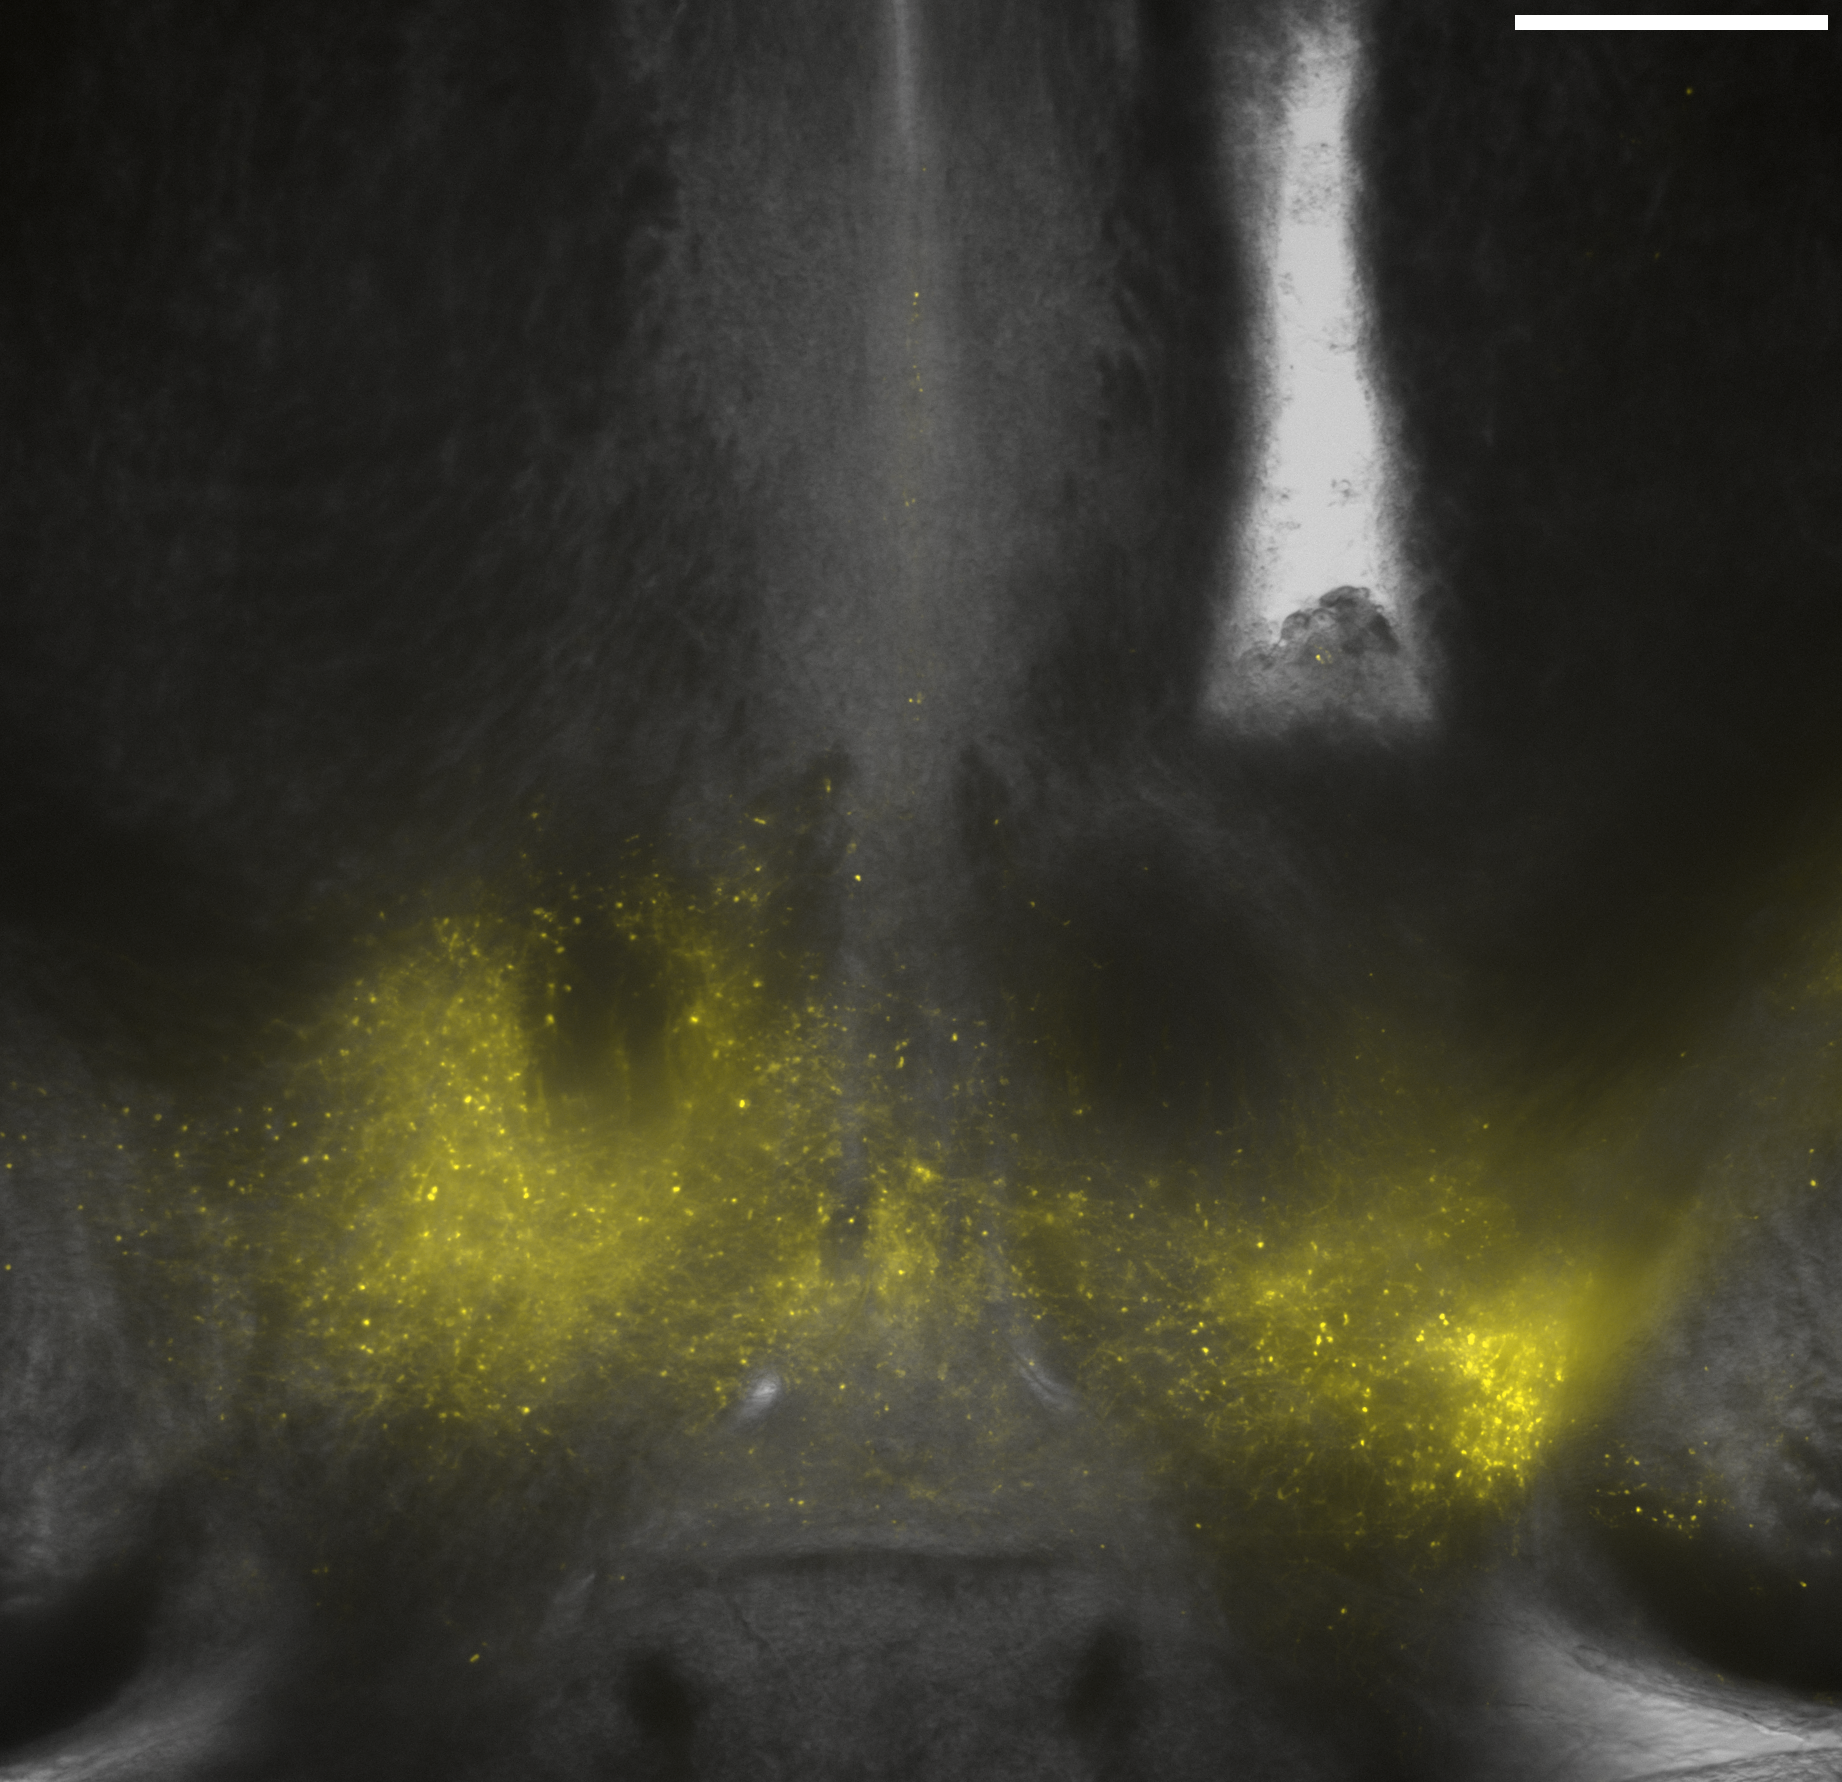
\includegraphics[width=\textwidth]{img/sub-6591_slice-b1_zoom-5_scene-3_transmission-yfp-comb_straight.png}
                \caption{\SI{3.05}{\milli\meter} caudal of Bregma.}
                \label{fig:h6591}
	\end{subfigure}
	\begin{subfigure}{.43\textwidth}
		\centering
		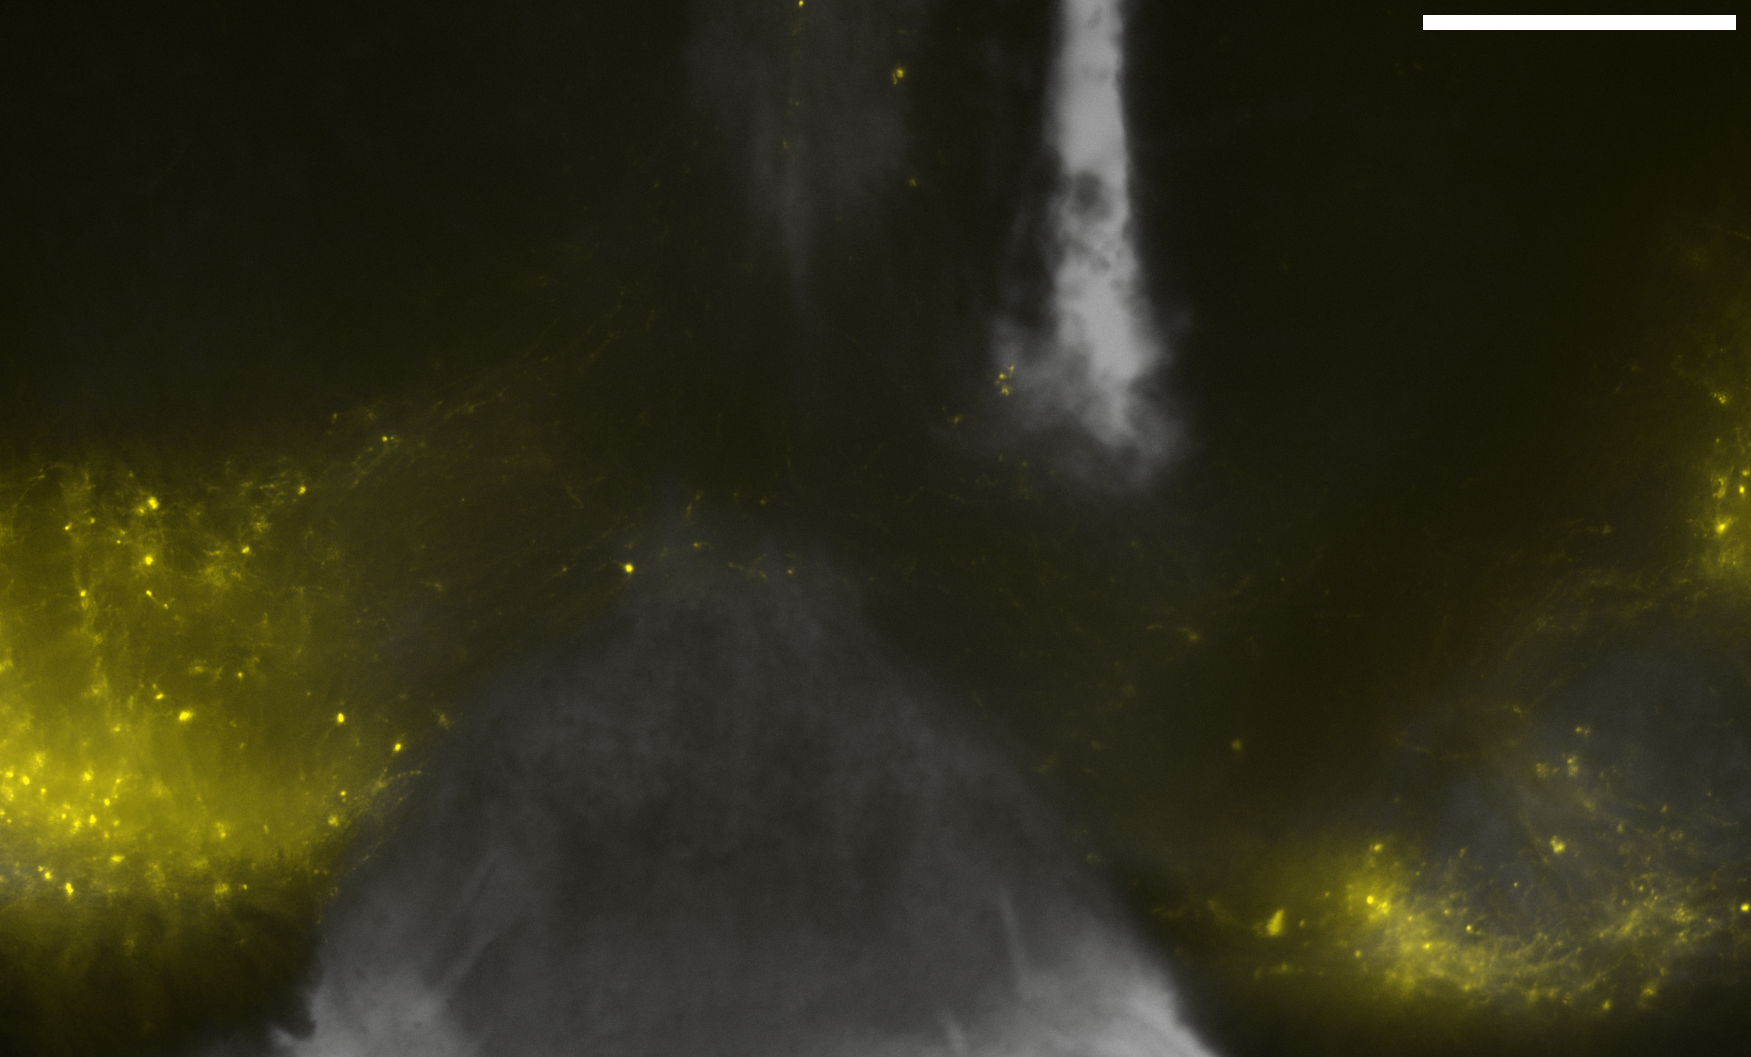
\includegraphics[width=\textwidth]{img/sub-6589_slice-a4_zoom-5_scene-2_transmission-yfp-comb_straight.png}
                \caption{\SI{3.5}{\milli\meter} caudal of Bregma.}
		\label{fig:h6589}
	\end{subfigure}
	\begin{subfigure}{.2728\textwidth}
		\centering
		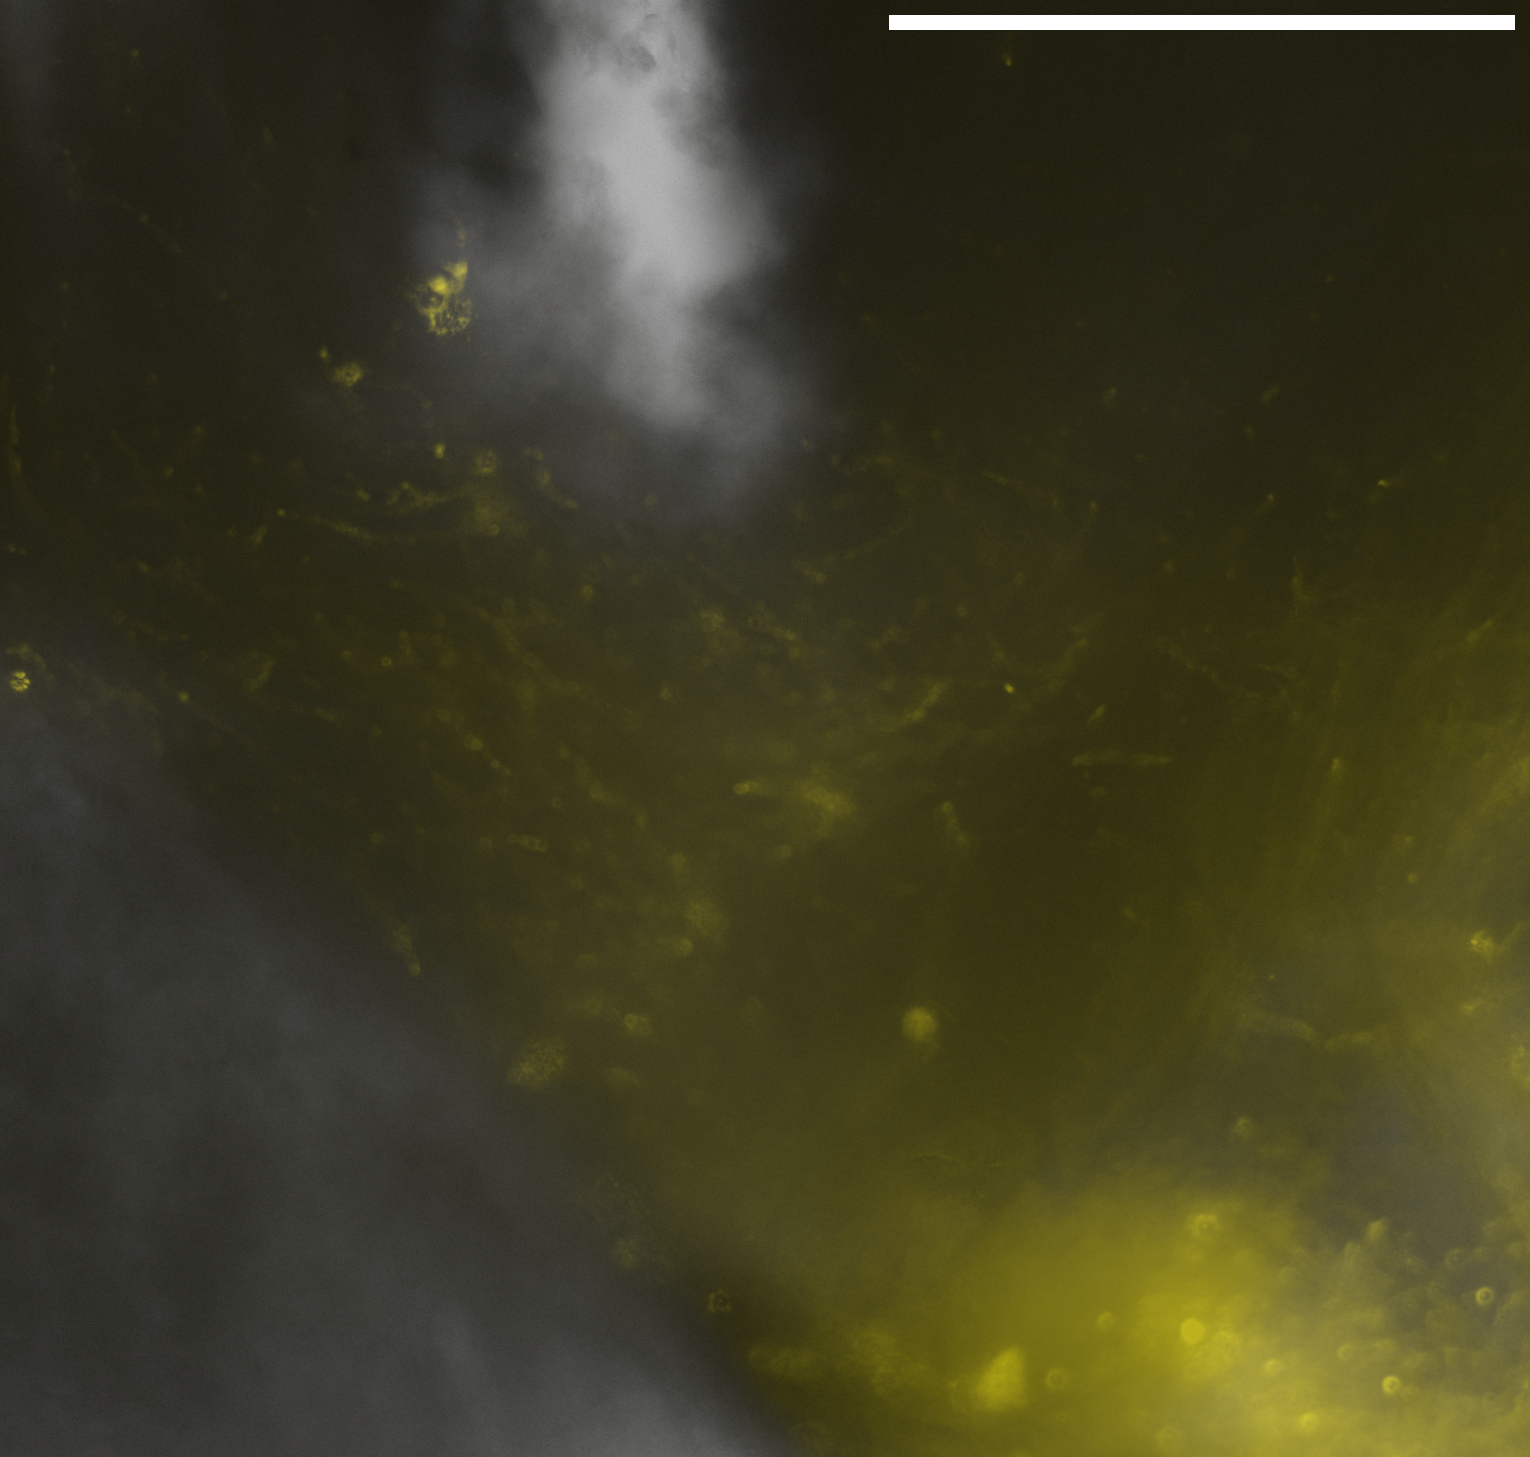
\includegraphics[width=\textwidth]{img/sub-6589_slice-a4_zoom-10_scene-2_transmission-yfp-comb_straight.png}
                \caption{\SI{3.5}{\milli\meter} caudal of Bregma.}
		\label{fig:h6589z}
	\end{subfigure}
        \vspace{-.5em}
	\caption{
		\textbf{Fiber implantation causes strong local cell displacement in the VTA.}
                Depicted are YFP (coexpressed with Channelrhodopsin) fluorescent microscopy images of the VTA, overlaid on corresponding transmission microscopy images of the same focal plane.
                All slices are seen in neurological orientation (the right of the image corresponds to the right of the animal).
                A higher magnification of \textbf{(\subref{fig:h6589})} is depicted in \textbf{(\subref{fig:h6589z})}.
                White bars indicate a scale of \SI{500}{\micro\meter}, and slices are shown in neurological orientation.
                }
	\label{fig:h}
\end{figure*}

Opto-fMRI experiments were carried out in C57BL/6 mice expressing Cre recombinase under the dopamine transporter promoter \cite{dat}, with Cre-conditional viral vector induced expression of channelrhodopsin (ChR2) and yellow fluorescent protein (YFP) in the dopaminergic midbrain.
Light stimuli were delivered via an optic fiber pointing above the right VTA.
Different stimulation protocols were applied to the animals, consisting of variations within two main categories:
block stimulation (with light stimuli delivered in continuous blocks of at least \SI{8}{\second} --- \cref{tab:CogB,tab:CogBr,tab:CogBl,tab:CogBm,tab:CogMwf})
and
phasic stimulation (with light stimuli delivered in short bursts of up to \SI{1}{\second} in lenght --- \cref{tab:CogP,tab:JPogP}).
Additionally, the dataset details the effects of variation in the posteroainerior (PA) coordinates and the implant depth (equivalent to the dorsoventral coordinate of the fiber endpoint), specified relative to bregma and the skull surface, respectively.

In the analysis of the resulting data, the mean t-statistic for the stimulation regressor fit across the VTA region of interest is found sensitive to
the stimulation protocol category (\sessionpy{boilerplate.anova(factor='Q("Task Category")')}),
the stimulation target depth (\sessionpy{boilerplate.anova(factor='C(Q("Depth rel. skull [mm]"))')}),
% Results before methods:
%the stimulation target posteroanterior (PA) coordinates (\sessionpy{boilerplate.anova(factor='C(Q("PA rel. Bregma [mm]"))')}),
the stimulation target PA coordinates (\sessionpy{boilerplate.anova(factor='C(Q("PA rel. Bregma [mm]"))')}),
but not the interaction of the depth and PA target coordinates (\sessionpy{boilerplate.anova(factor='C(Q("Depth rel. skull [mm]")):C(Q("PA rel. Bregma [mm]"))')}).

The break-up by phasic and block stimulation is shown in \cref{fig:mv} and significance is evaluated accounting for the entire statistical model, consisting of categorical terms for both the stimulus category and the coordinates.
The phasic and block levels of the stimulation variable yield p-values of
$\sessionpy{boilerplate.posthoc_t('Q("Task Category")[Phasic]')}$
and
$\sessionpy{boilerplate.posthoc_t('Q("Task Category")[Block]')}$,
respectively.
Upon investigation of the t-statistic map, phasic stimulation further reveals no coherent activation pattern at the whole-brain level(\cref{fig:phasica}).

The main and interaction effects of the implant coordinate variables are better described categorically than linearly (\cref{fig:mvs,fig:mvib}).
Consequently, the most suitable implant coordinate group for the assay can best be determined on the basis of categorical classification of implant coordinates.
We classify the implant coordinates into a “best” and a “rejected” group by k-means clustering the aggregate VTA t-statistic scores into two clusters, and find spatial coherence for the “best” coordinate group (categorization highlighted in \cref{fig:mvib}).

For block stimulation, the best implant category group (\cref{fig:mbfc}) and the rejected implant category group (\cref{fig:mboc}) show not only a difference in overall stimulus-evoked signal intensity, but also a difference in efferent distribution, with the rejected implant category efferent spectrum more strongly weighted towards caudal brain areas.
This distinction specifically arises for implant categorization based on block scan VTA t-statistic means, and is not as salient if implants are categorized based on a posteroanterior implant coordinate delimiter (\cref{fig:oc}).

The activation pattern elicited by block stimulation in the best implant category group shows strong coherent clusters of activation.
The top activation areas are predominantly located in the right hemisphere, with
highly significant laterality ($p = \sessionpy{boilerplate.lateral('data/l2/alias-block_filtered_controlled/acq-EPI_tstat.nii.gz')}$) seen in the comparison of left and right hemisphere atlas parcellation region averages.
Activation is seen in regions surrounding the stimulation site, such as the ventral tegmental decussation and the interpeduncular nucleus.
The largest activation cluster encompasses well-known dopaminergic VTA projection areas in the subcortical rostroventral regions of the brain (nucleus accumbens, striatum, and the basal forebrain), with weaker activation observed in smaller structures in the vicinity of these regions, such as the fasciculus retroflexus, anterior commissure and the claustrum.

This activation pattern is is largely consistent with structural projection data, as published by the Allen Brain Institute \cite{abic} with a few notable distinctions (\cref{fig:f}).
At the parcellation level, we see a moderately strong positive correlation between functional activation and structural projection (\cref{fig:fcr}), which is weaker at the voxel level (\cref{fig:fcv}).
In the midbrain, the coronal slice map shows areas of increased functional activation with respect to structural projection density in the contralateral VTA and the ipsilateral substantia nigra.
Coherent clusters of increased activation are also observed in projection areas, most prominently in the ipsilateral and contralateral dorsomedial striatum (\cref{fig:ffc}).
Parcellation-based distributions (\cref{fig:dffp,fig:dffn}) show this increased activation map encompassing additional areas in the contralateral hemisphere, in particular the contralateral nucleus accumbens, with activity extending into the claustrum.
%% Should we keep this?
%%The pattern of increased activation thus includes all regions with dense structural projections.
Areas for which structural projections clearly outweigh the functional response are few and dispersed.
These small clusters yield only weak negative contrast distributions and are located predominantly in the cerebellum (\cref{fig:dffn}).
%These small clusters amount to weak negative contrast distributions in regions such as the cerebellum, the olfactory bulb, and the amygdaloid area (\cref{fig:dffn}).

We differentiate VTA transmission from VTA excitability by mapping functional connectivity using a seed region in the right VTA, which yielded the projection pattern shown in \cref{fig:mbfs}.
These clusters are more sparse compared to those identified by stimulus-evoked analysis, yet follow a similar distribution.
While areas displaying the highest functional connectivity are located in the right hemisphere, the whole brain parcellation-resolved response displays
no significant laterality ($p = \sessionpy{boilerplate.lateral('data/seed_l2/alias-block_filtered/acq-EPI_tstat.nii.gz')}$).
Strong activation can be seen in the parcellation regions surrounding the seed, such as the ventral tegmental decussation and the closely located interpeduncular nucleus.
In the midbrain, seed-based functional connectivity highlights both the ipsilateral and the contralateral VTA with great specificity, unlike sitmulus-evoked analysis (\cref{fig:mbfs,fig:mbfc}).
Rostrovental dopaminergic projection areas remain prominently featured, including the nucleus accumbens and the striatum (\cref{fig:dbfs}).

Stimulation in wild type control animals (which is corrected for in the aforementioned stimulus-evoked analyses) does not exhibit a pattern of activity consistent with dopaminergic projections.
Sparse grains containing regression scores of $t \geq 3$ can be observed, with the largest cluster in the lateral geniculate nucleus area of the thalamus, suggesting visual activity (\cref{fig:control_mapa}).
Atlas parcellation score distributions (\cref{fig:control_dist}) do not strongly deviate from zero, with the highest scoring areas being in the vicinity of the fiber, possibly indicating VTA heating artefacts.
Comparable region t-statistic distributions are also found in areas of the cerebellum.
Overall the whole brain parcellation-resolved response shows
no significant laterality ($p = \sessionpy{boilerplate.lateral('data/seed_l2/alias-block_control/acq-EPI_tstat.nii.gz')}$).

Histological analysis of the targeting site reveals that the optic fiber implant displaces the YFP labelled neurons of the VTA (\cref{fig:h}).
This dislocation was observed irrespective of the targeting area or the speed of implant insertion (\SIrange{10}{50}{\micro\meter\per\second}).
Yet, labelled filaments and soma remain in the imediate vecinity of the fiber tip, as seen in higher magnification images (\cref{fig:h6589z}).
